\section{PERFORMANCE BENCHMARKS}

In this section, we provide a number of performance benchmarks. The tests are running on a Dell Precision 7740 Workstation Laptop with 64 GB RAM. Its CPU is an Intel i9-9980HK with a base clock of 2.4GHz and a burst clock of 5GHz. The CPU supports AVX, AVX2, and AVX-512.
As a GPU we use an Nvidia RTX 3000 GPU. All benchmark tests were performed in Linux. For OpenCL on the GPU, we use the Nvidia GPU drivers and as CPU runtime we compare the open-source PoCL driver against the Intel CPU OpenCL runtime environment. All timing runs were repeated several times to make sure that the overhead from running the OpenCL and Numba JIT compilers did not skew the results. Though hardly noticeable by users, for smaller experiments the JIT phase typically takes longer than the actual computation.

\subsection{Dense Operator assembly}
We start by benchmarking the dense operator assembly. We assemble the matrix $\dmat{A}$ defined by
$$
\dmat{A}_{ij} = \int_{\Gamma}\psi_i(\bx)\int_{\Gamma}\frac{\phi_j(\by)}{4\uppi |\bx -\by|}\ds[\by]\ds[\bx],
$$
with $\Gamma$ being the unit sphere. For the basis functions $\phi_j$ and test functions $\psi_i$, we compare two cases: piecewise constant functions for both (P0 functions); and nodal, piecewise linear, and globally continuous functions for both (P1 functions). In the P0 case, each triangle is associated with just one piecewise constant function. In the P1 case, each triangle is associated with $3$ linear basis functions, one for each node of the triangle.

We first compare the OpenCL CPU performance for the Intel OpenCL runtime, and the PoCL OpenCL runtime driver. We run the tests in single precision and double precision. The native vector width for both drivers in single precision is $8$, and in double precision is $4$, which corresponds to AVX instructions. In Bempp-cl, this means that we assemble in vectorized form one test triangle with $8$ trial triangles in single precision, and with $4$ trial triangles in double precision. Within the assembly, almost all floating point instructions are manually vectorized to take advantage of this. We should hence see up a factor 2 speed-up between single and double precision assembly.

\begin{figure}
	\center
	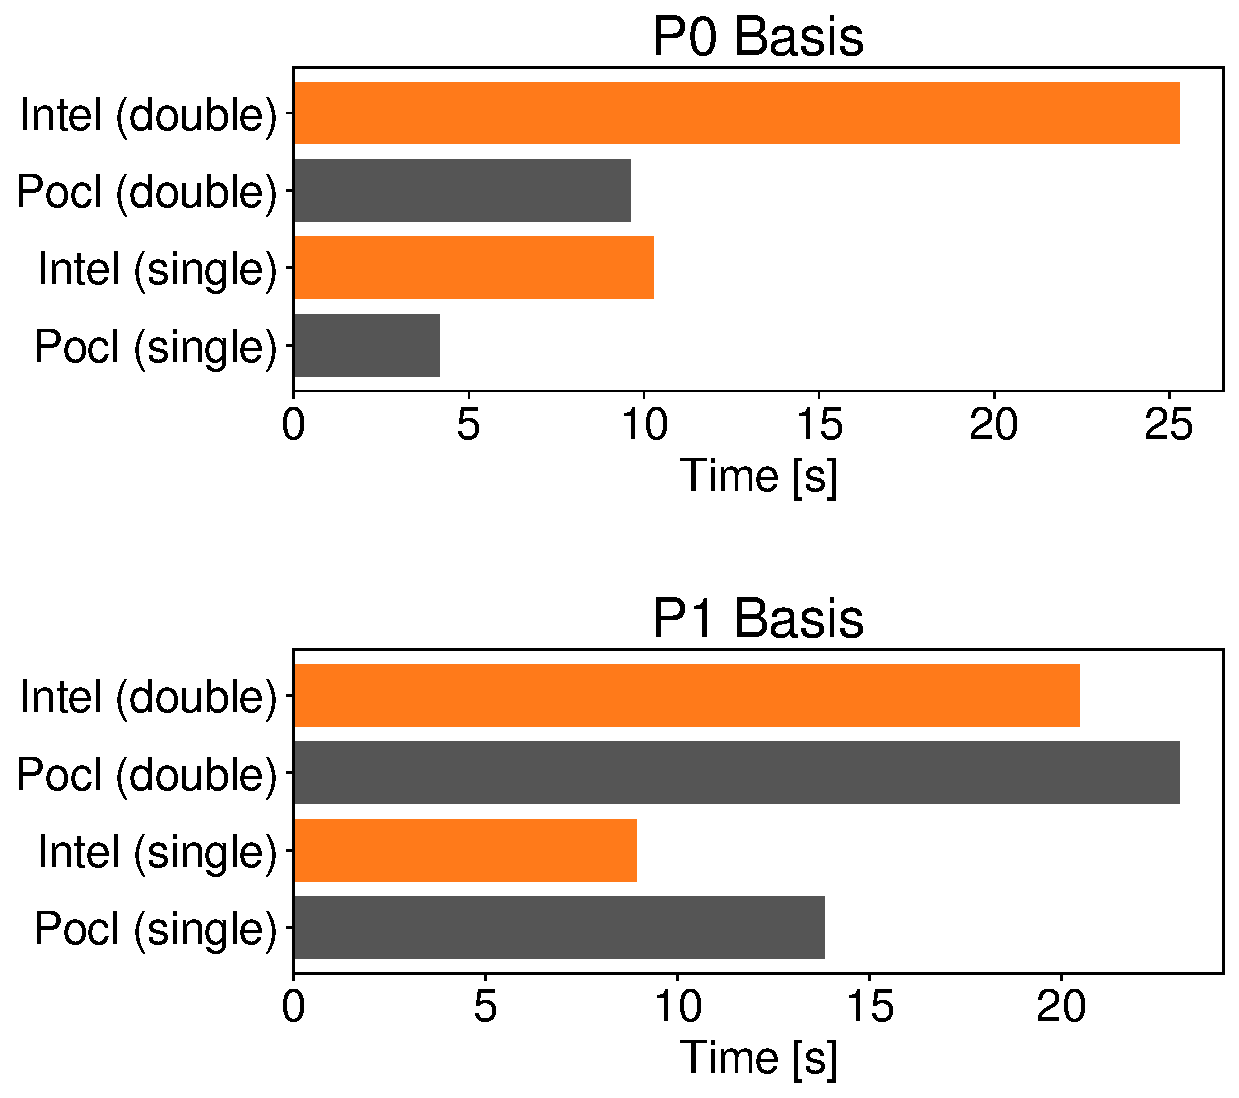
\includegraphics[width=6cm]{img/intel_pocl_laplace_comp.pdf}
	\caption{Comparison of the performance of PoCL and the Intel OpenCL runtime for the assembly of the Laplace single-layer boundary operator on a grid with 32,768 elements.}
	\label{fig:intel_pocl_laplace_cmp}
\end{figure}

The timings for a grid with 32,768 elements are shown in \cref{fig:intel_pocl_laplace_cmp}. We see the expected speed-up between single precision and double precision evaluation. It is interesting to note the difference between the Intel and the PoCL runtime environment. For P0 basis functions, the PoCL driver (gray bar) significantly outperforms the Intel driver (orange bar) in both single and double precision. For P1 basis functions, however, the Intel driver gives better performance. The kernel source code is the same in both cases and manual vectorization of floating point operations is performed in the same way. In the P1 case, significantly more data needs to be copied between a work-item and the global memory since the result of the interaction of a test triangle with a trial triangle is a local $3\times 3$ matrix containing all interactions between the three test basis functions on a triangle and the three trial basis functions. {\color{red}(?)}

In \cref{fig:pocl_single_layer}, we compare specifically the performance of single precision and double precision evaluation for the PoCL driver for various grid sizes in the case of a P0 basis. We can see that the speed-up for larger grid sizes is slightly more than just a factor of two. The final data point in this graph corresponds to the grid size used for \cref{fig:intel_pocl_laplace_cmp}.

\begin{figure}
	\center
	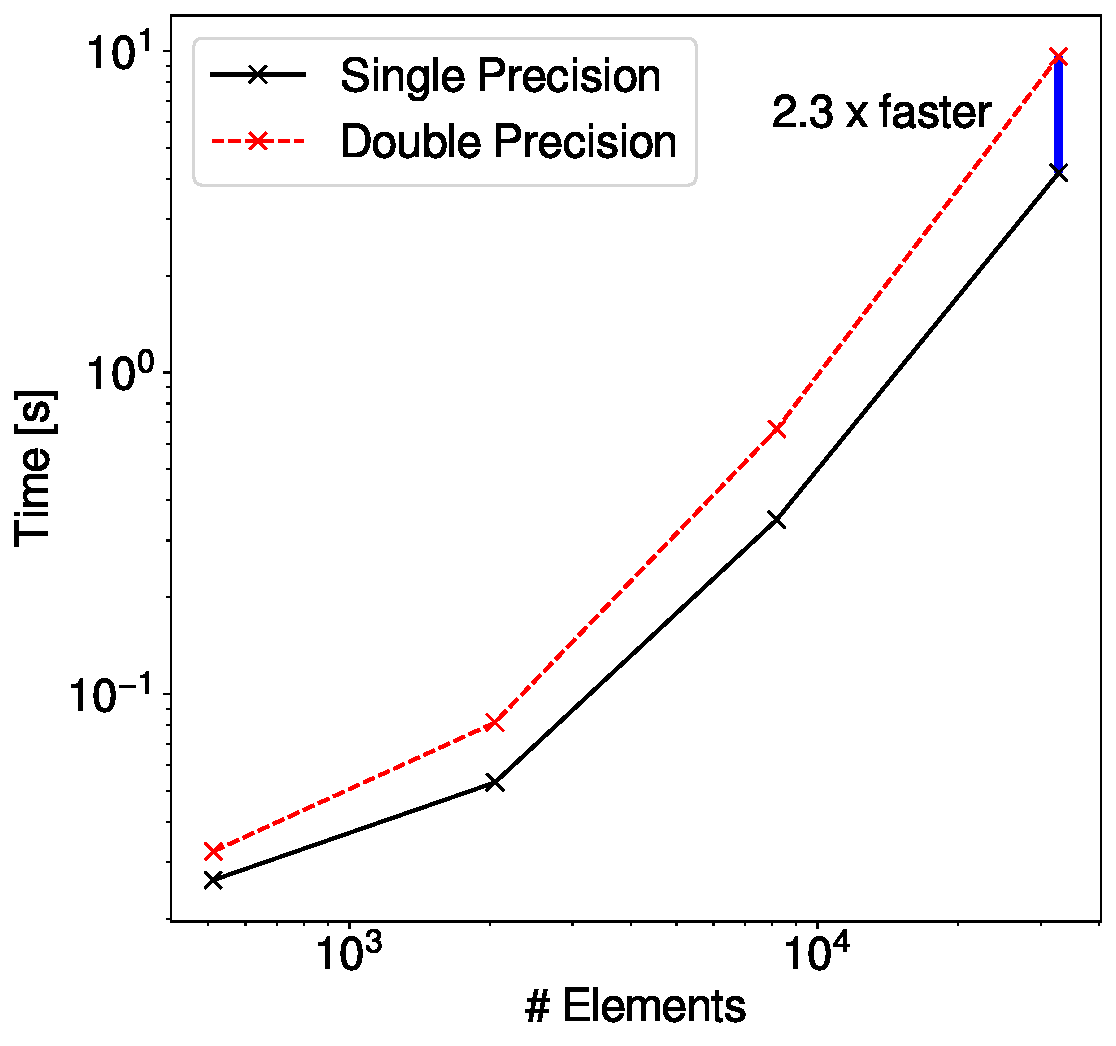
\includegraphics[width=7cm]{img/pocl_single_layer.pdf}
	\caption{Comparison of the single-precision and double-precision performance for various grid sizes using PoCL and P0 basis functions.}
	\label{fig:pocl_single_layer}
\end{figure}

\begin{figure}
\begin{center}
\begin{tabular}{l|c|c}
	        &   single      &    double\\
	        \hline
	 PoCL   &   0.05s       &    0.08s\\
	 Numba  &   0.25s       &    0.25s\\
	 GPU    &   0.11s       &    3.00s\\
\end{tabular}
\end{center}
\caption{Comparison of PoCL, Numba and GPU Assembly for a grid with 2048 elements.}
\label{fig:cpu_gpu_numba_compare}
\end{figure}
In Bempp-cl, we can easily switch between CPU Assembly, GPU Assembly, and Numba Assembly. \Cref{fig:cpu_gpu_numba_compare} shows a comparison between these modes for a grid with 2048 elements. The speed differences are striking. GPU assembly in single precision is a factor of two slower than CPU assembly (and much slower in double precision due to Nvidia hardware restrictions for double precision). Numba is five times slower for single precision and still around three times slower for double precision than PoCL. The GPU behaviour can be explained by data transfer: while the GPU kernels themselves are extremely fast, data transfer over the bus severely limits performance. Even for medium sized problems, we have to transfer the data back to the main memory as GPU RAM is too limited to keep dense matrices with a tens of thousands or rows and columns on the device.

An alternative method is to compute the matrix-vector product (matvec) $\dmat{A}\dvec{x}$ on the device without first computing the dense matrix $\dmat{A}$. This can be done by recomputing all matrix elements during each matvec calculation on-the-fly and not storing them. We have done experiments with this, and observed significant speed-ups compared to CPU evaluation as we now only need to transfer single vectors over the bus. For larger problems, however, it is not competitive compared to accelerated methods such as fast multipole methods (FMM), due to the quadratic complexity of direct evaluation of the matvec compared to linear complexity of FMM. For smaller problems, it is still practically better to just assemble the whole matrix and store it, as then matvecs are much faster for an iterative solver. Hence, we can conclude that there is only limited practical relevance for on-the-fly GPU evaluation of boundary integral operators. There are, however, very significant practical advantages of on-the-fly evaluation of the evaluation of domain potential operators for visualization and post-processing, as we will see in the next section.

The Numba performance difference seen in \cref{fig:cpu_gpu_numba_compare} is interesting. The main reason for this, we believe, is significantly lower usage of AVX vectorized instructions. We have taken care to optimize the Green's function evaluation for auto-vectorized evaluation in Numba, but the loops over integration points and other operations auto-vectorize very badly when just looping over all trial triangle for a single test triangle, as we currently do. We could tune our code for better auto-vectorization in Numba, but this would give little benefit as we have highly optimized hand-tuned OpenCL kernels already. We therefore recommend using Numba for operator assembly only as a fallback if no OpenCL runtime is available.

\subsection{Evaluating domain potentials for post-processing of electromagnetic problems}
Once an integral equation is solved, one is usually interested in evaluating the solution not only at the boundary but also at points away from it. To do this, we evaluate the integral
$$
f(\bx) = \int_{\Gamma}g(\bx, \by)\phi(\by) \ds[\by]
$$
for many points $\bx$ away from the boundary $\Gamma$. For example, if we want to visualize a solution, we take the points $\bx$ to be a regular grid of points.

Typically, we want to do only a small number of potential evaluations at the end of a calculation. Discretising this operation into a dense matrix and then evaluating the dense matrix-vector product is not practical for larger sizes. For very large problems with hundreds of thousands of elements, we use FMM or other accelerated approximate methods. For moderately sized problems with a few ten thousand elements up to around a hundred thousand elements (depending on the problem at hand), direct evaluation of this integral for every point $\bx$ is highly efficient. We won't go into the details of the corresponding OpenCL kernels here, but we show some results that demonstrate the relative performance on CPUs and GPUs.

For the dense assembly of boundary integral operators, the performance was limited by the bus transfer of the dense matrix. For the evaluation of domain potentials, however, we only need to transfer to the device the vector of coefficients of the basis functions for $\phi$, and then transfer back to the host the values at the points $\bx$.

In this section, we consider the evaluation of the electric potential operator, defined by
\begin{multline}
\left(\mathcal{E}\mathbf{p}\right)(\bx) = \ii k\int_{\Gamma}\mathbf{p}(\by)g(\bx, \by) \ds[\by]\\
-\frac{1}{\ii k}\nabla_{\bx}\int_{\Gamma}\operatorname{div}\mathbf{p}(\by)g(\bx, \by)\ds[\by],
\end{multline}
where $g(\bx, \by) = \frac{\ee^{\ii k|\bx - \by|}}{4\pi|\bx - \by|}$ is the Helmholtz Green's function, and
$k$ the wavenumber of the problem.
The function $\mathbf{p}:\mathbb{R}^3\to\mathbb{R}^3$ is a vector-valued function, leading to an overall vector solution at each point $\bx$. The implementation of electromagnetic problems in Bempp is covered in detail in \cite{bempp_maxwell}. For these experiments, we again use a grid with 32,768 elements and RWG (Rao, Wilton, and Glisson) edge-based basis functions. For the potential evaluation, we use 50,000 random evaluation points in the exterior of the unit sphere. We set $k=1.0$, although the wavenumber have little to no effect on the performance. {\color{red}[If $k$ is very high, surely it becomes relevant?]}

In \cref{fig:efield_domain_potential}, we compare the performance of GPU evaluation with that of the PoCL CPU driver. In single-precision, the GPU significantly outperforms the CPU; and even in double-precision, the Quadro {\color{red}[Quadro? Nvidia?]} RTX GPU is faster than the 8-core CPU, even though its hardware is not optimised for fast double-precision operations.

\begin{figure}
	\center
	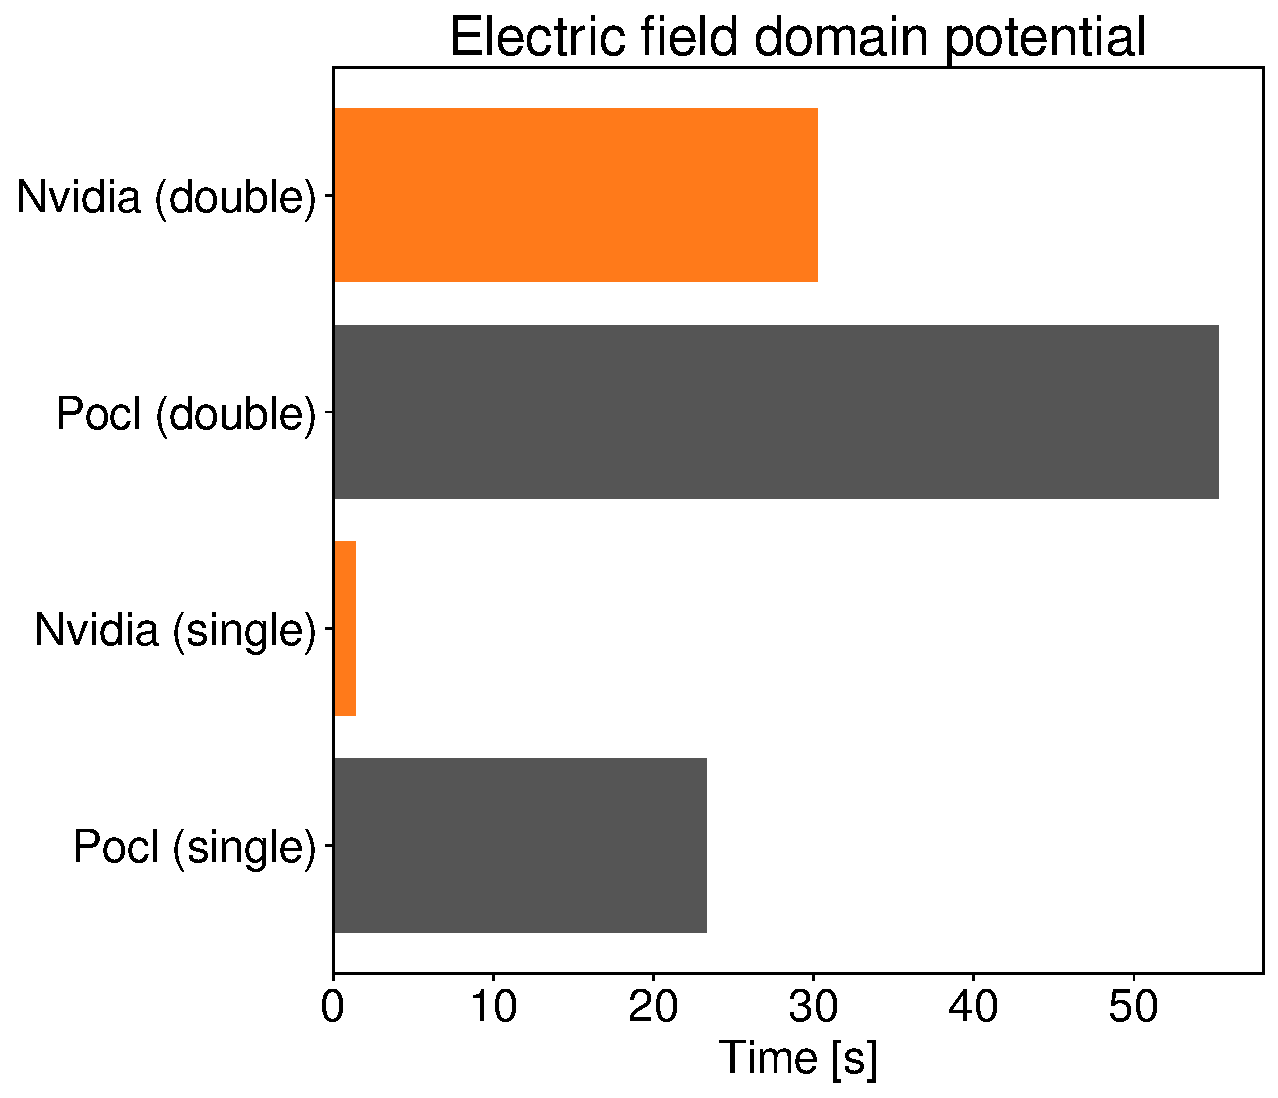
\includegraphics[width=7cm]{img/efield_domain_potential.pdf}
	\caption{Evaluation of an electric field potential operator on CPU via PoCL vs GPU}
	\label{fig:efield_domain_potential}
\end{figure}

\section{SUMMARY}
With Bempp-cl, we have created a Python library that achieves high-performance through use of modern just-in-time compilation technologies. Bempp-cl mixes Numba evaluation for less compute intensive linear complexity loops and sparse matrix generation with highly optimized OpenCL kernels for computationally sensitive dense matrix assembly routines. Basing development in Python instead of classical C/C++ makes it very easy to adapt the library and integrate with other libraries with Python interfaces, such as the recent work integrating Bempp-cl and the Exafmm library to build electrostatic virus-scale simulations \cite{bempp_exafmm}.

Strict separation of the computational backend from the interface layer in the library also makes it easy to integrate further backends, allowing us to remain up to date with future compute models. OpenCL itself has proved a valuable choice for the purpose of this library, as it allows us to run CPU and GPU optimized kernels with very little code overhead, and allows the user to easily move between CPU and GPU based compute devices with a simple parameter change. In this article, we demonstrated Nvidia benchmarks, the same benchmarking code could be used to run on AMD or Intel GPUs (for example).

A disadvantage of our approach is that using OpenCL kernels introduce a second language (C99) to the library. Using Numba throughout would give a much more native Python experience, but, while Numba is constantly improving, it is currently difficult to achieve optimal performance for complex operations. OpenCL really shines here, as it makes explicit SIMD operations very easy through dedicated constructs. Moreoever, OpenCL kernels are completely stack based functions, allowing much better compiler optimisations while Numba needs to create every object dynamically, even very small arrays for objects such as coordinate vectors.

Additionally, one has to consider the type of operations that need to be accelerated. For the dense assembly of integral operators, we have very simple data structures that can easily be passed to compute kernels. More complex data structures with larger mixture of data movement operations and computations (e.g., tree-based algorithms), are much harder to accelerate since the Python layer imposes limits here on the performance.

Overall, with the model of mixed Python/OpenCL/Numba development, we have created a flexible and easy to extend platform for integral equation computations. The initial re-implementation efforts are really paying off, as they allow us to develop new features in a far simpler environment without sacrificing performance. Strict separation of compute backends and higher level routines makes it easy for us to integrate other accelerator techniques in the future with little code changes, and to react to new trends in heterogeneous computing.

The current focus of further developments is on letting Bempp-cl take advantage of cluster computing by integrating the \pyth{mpi4py} MPI bindings for Python. We have also made big steps forward for large problems by creating a black-box FMM interface that currently intenfaces to Exafmm: this has allowed us to solve problems with 10 million elements on a single workstation. We believe that Python-focused development (with some native routines in lower-level languages) is a scalable model and are aiming to exploit this scalability further as we move from single workstation computations to large cluster problems.

\section{Acknowledgements}
The work of Timo Betcke is supported by Engineering and Physical Sciences Research Council Grant EP/V001531/1.
